\documentclass[12pt,letterpaper]{article}
\usepackage[latin1]{inputenc}
\usepackage[spanish]{babel}
\usepackage{graphicx}
\usepackage[left=2cm,right=2cm,top=2cm,bottom=2cm]{geometry}
\usepackage{graphicx} % figuras
\usepackage{subfigure} % subfiguras
\usepackage{float} % para usar [H]
\usepackage{amsmath}
\usepackage{txfonts}
\usepackage{stackrel} 
\usepackage[latin1]{inputenc}
\usepackage{multirow}
\usepackage{enumerate} % enumerados
\renewcommand{\labelitemi}{$-$}
\renewcommand{\labelitemii}{$\cdot$}
\author{Nelia Escalante}
\title{Caratula}
\begin{document}

\title{Caratula}

\begin{titlepage}
\begin{center}
\large{UNIVERSIDAD PRIVADA DE TACNA}\\
\vspace*{-0.025in}
\begin{figure}[htb]
\begin{center}

\includegraphics[width=11cm]{./IMG/logo}
\end{center}
\end{figure}
\Large INGENIERIA DE SISTEMAS  \\

\vspace*{0.5in}
\begin{large}
\textbf{TITULO:} \\
\end{large}

\vspace*{0.1in}
\begin{Large}
\textbf{Elaboracion de Dashboards en Power BI} \\
\end{Large}

\vspace*{0.3in}
\begin{Large}
\textbf{CURSO:} \\
\end{Large}

\vspace*{0.1in}
\begin{large}
INTELIGENCIA DE NEGOCIOS\\
\end{large}

\vspace*{0.3in}
\begin{Large}
\textbf{DOCENTE:} \\
\end{Large}

\vspace*{0.1in}
\begin{large}
 Ing. Patrick Cuadros Quiroga\\
\end{large}

\vspace*{0.2in}
\vspace*{0.1in}
\begin{large}
\textbf{ESTUDIANTE:} \\
\vspace{\baselineskip}
\begin{flushleft}

Escalante Maron, Nelia 		\hfill	(2014049551) \\

\end{flushleft}
\end{large}
\end{center}

\end{titlepage}

\newpage

	\begin{center}
		\Large ELABORACION DE DASHBOARDS EN POWER BI
	\end{center}
	\vspace{\baselineskip}
	\vspace{\baselineskip}
	\textbf{\Large 1. RESULTADOS DEL DESARROLLO:}
	\\\\
Al desarrollar los pasos anteriores de la practica, veremos y mostraremos los resultados siguientes, indicando los pasos que se desarrollaron. \\\\


1. Iniciar Power BI Desktop.\\\\ 
2. Cuando la Ventana de Power BI Desktop aparezca, en el panel a mano izquierda, hacer click en Obtener Datos (Get Data).\\\\ 
3. En el cuadro de dialogo Obtener Datos (Get Data), click en base de datos SQL Server, y luego hacer click en Conectar (Connect).\\\\ 
4. En el cuadro de dialogo base de datos SQL Server, en la casilla servidor tipear (local), en la casilla Base de datos (opcional) / Database (optional), tipear AdventureWorks2017, y hacer clic en OK.\\\\ 
\begin{center}
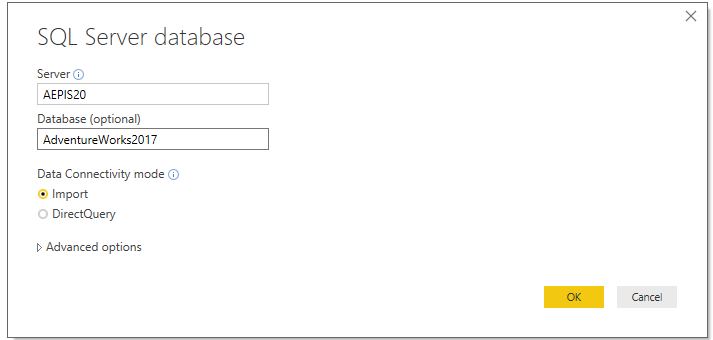
\includegraphics[width=11cm]{IMG/1.png} 
\end{center}
5. En el cuadro de dialogo base de datos SQL Server, aceptar los valores por defecto, y luego click en el Conectar (Connect). Si un mensaje de Soporte de Encriptacion es visualizado, hacer click en OK.\\\\ 
\begin{center}
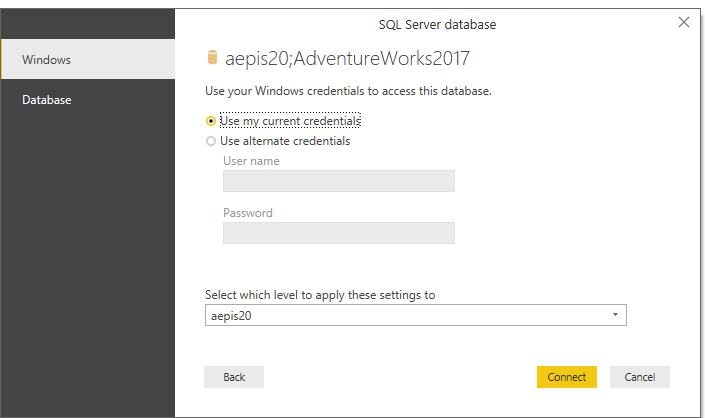
\includegraphics[width=11cm]{IMG/2.png} 
\end{center}
6. En el cuadro de dialogo Navegador (Navigator), seleccionar el check en Sales.vSalesPerson, y entonces hacer click en Cargar (Load).\\\\ 
7. En el panel Campos (Fields), expandir Sales vSalesPerson para ver todas las columnas.\\\\ 
8. En el menu principal (Home ribbon), hacer click en Funetes Recientes (Recent Sources), y en local: AdventureWorks2017.\\\\ 
9. En el cuadro de dialogo Navegador (Navigator), seleccionar la vista Sales.vStoreWithDemographics, y luego
hacer click en Cargar (Load).\\\\ 
10. En el panel Campos (Fields), expandir Sales.vStoreWithDemographics para ver todas las columnas.\\\\ 
11. En el menu principal (Home ribbon), hacer click en Obtener Datos (Get Data), y luego click en SQL Server.\\\\ 
12. En el cuadro dialogo base de datos SQL Server, en la casilla Servidor (Server), tipear (local), y en la casilla
Base de datos (opcional), tipear AdventureWorks2017.\\\\ 
13. Expandir opciones Avanzadas, en la casilla sentencia SQL (opcional, base de datos requerida), tipear la
siguiente consulta, y luego hacer click en OK:\\\\ 
14. Si la Ventana Configuracion de la Conexion (Connection Settings) aparece, hacer click en OK.\\\\ 
15. En el cuadro de dialogo (local): AdventureWorks2017 hacer click en Cargar (Load).\\\\ 
16. En el panel Campos, expander Query1 para ver todas las columnas.\\\\ 
\begin{center}
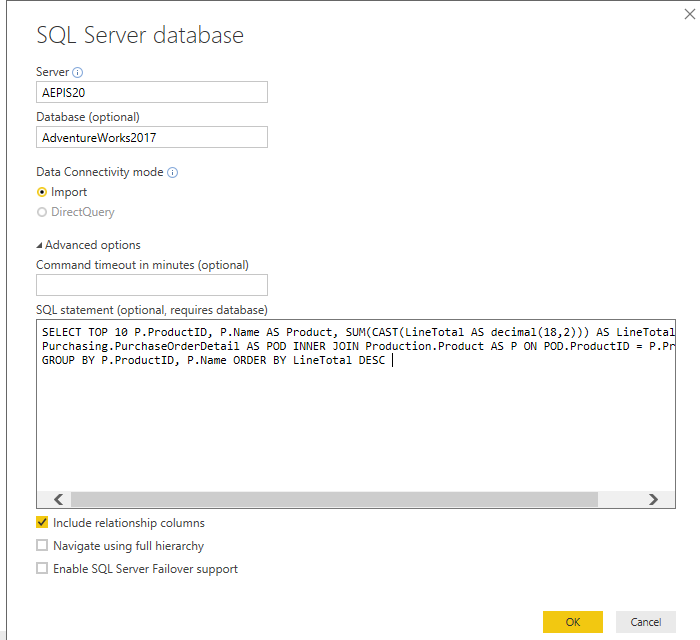
\includegraphics[width=11cm]{IMG/3.png} 
\end{center}

\begin{center}
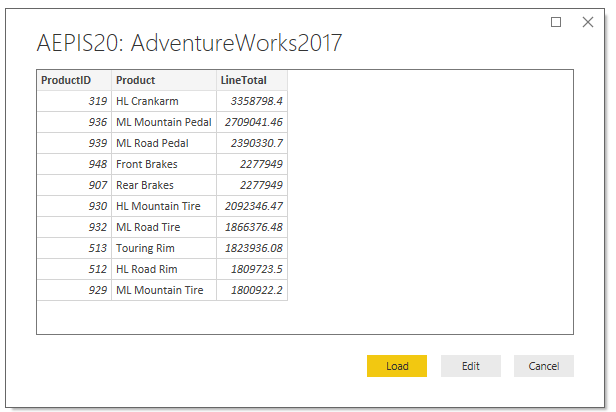
\includegraphics[width=11cm]{IMG/4.png} 
\end{center}
17. Hacer click en la elipsis al lado de Query1 y hacer click en Renombrar, tipear Top 10 Productos
Vendidos, y presionar Enter.\\\\
\begin{center}
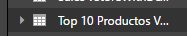
\includegraphics[width=9cm]{IMG/5.png} 
\end{center}

Parte 2: Adicionar Graficos al Reporte\\\\
1. En el panel Visualizaciones (Visualizations), hacer click en el grafico Columna apilada (Stacked column) para
anadir el control al reporte.\\\\
2. En el panel Campos (Fields), bajo Sales vSalesPerson, arrastrar el campo FirstName a la casilla Eje (Axis) en el
panel de Visualizacion (Visualizations).\\\\
3. Arrastrar el campo SalesYTD a la casilla Valores (Values). El gráfico se llenará con datos.\\\\
\begin{center}
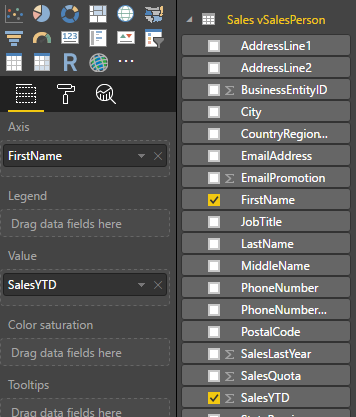
\includegraphics[width=10cm]{IMG/21.png} 
\end{center}
4. En el grafico en el reporte, ajustar el tamano del grafico para que muestre a todo el personal de ventas.\\\\
\begin{center}
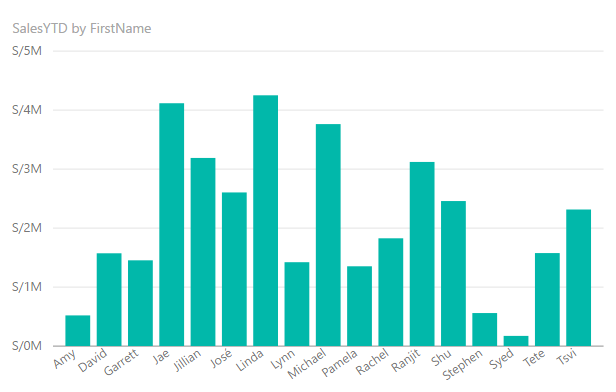
\includegraphics[width=11cm]{IMG/22.png} 
\end{center}
5. Asegurarse que el grafico tiene el foco y luego ir al panel de Visualizacion (Visualizations), hacer click en la
pestana Formato (Format).\\\\
\begin{center}
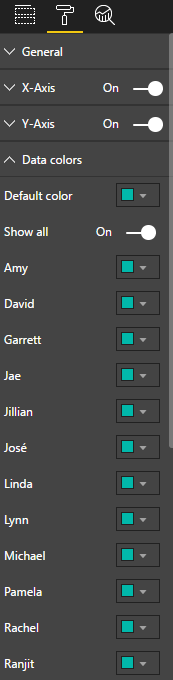
\includegraphics[width=3.5cm]{IMG/23.png} 
\end{center}
6. Expandir Colores de datos (Data colors), activar la opcion Mostrar todos (Show all).\\\\
7. Cambiar el color para Jae, Linda, y Michael a rojo.\\\\
\begin{center}
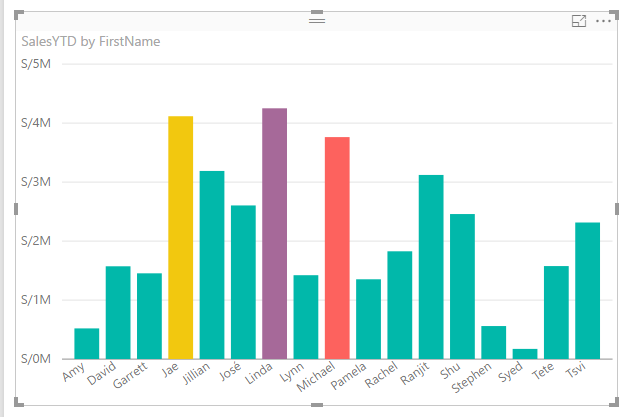
\includegraphics[width=11cm]{IMG/24.png} 
\end{center}
8. Hacer click en el area de reporte y luego en el panel de Visualizaciones (Visualizations pane), hacer clic en el
grafico Pie para anadir el control al reporte. Arrastrar el grafico Pie al lado derecho del grafico de barras o
debajo si no hubiese espacio.\\\\
\begin{center}
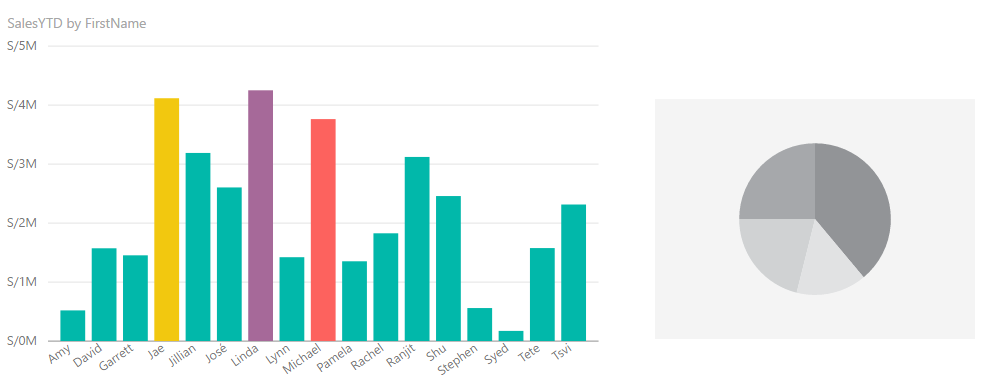
\includegraphics[width=14cm]{IMG/25.png} 
\end{center}
9. En el panel Campos (Fields pane), bajo Sales vStoreWithDemographics, arrastrar el campo Specialty a la
casilla Leyenda (Legend) en el panel de Visualizaciones.\\\\
\begin{center}
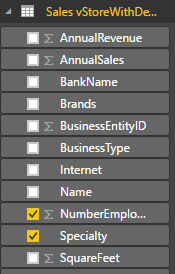
\includegraphics[width=5cm]{IMG/26.png} 
\end{center}
10. Arrastrar el campo NumberEmployees a la casilla Valores (Values). El grafico se llenara con los datos y
mostrara tres secciones.\\\\
\begin{center}
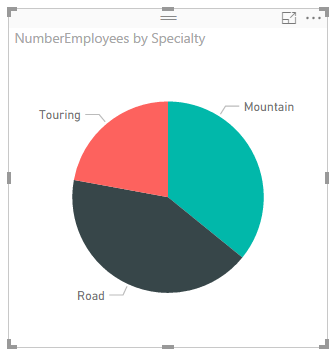
\includegraphics[width=11cm]{IMG/27.png} 
\end{center}
11. Nuevamente click en el area de reporte, luego ir al panel de Visualizaciones y anadir otro grafico de
Columna apilada (Stacked columna) al reporte. Este grafico debe estar debajo de los graficos previos.\\\\
12. En el panel Campos, expander Top 10 Productos Vendidos, arrastrar el campo Product a la casilla Eje (Axis)
en el panel de Visualizaciones.\\\\
\begin{center}
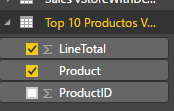
\includegraphics[width=7cm]{IMG/28.png} 
\end{center}
13. Arrastrar el campo LineTotal a la casilla Valores (Value). El grafico se llenara con datos.\\\\
\begin{center}
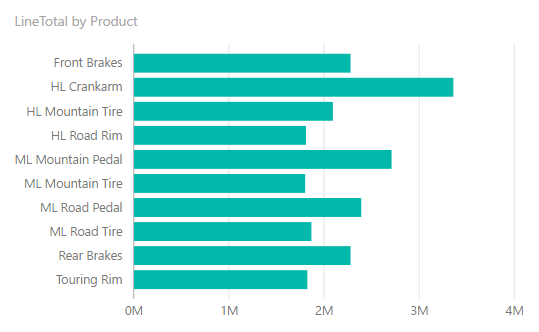
\includegraphics[width=13cm]{IMG/29.png} 
\end{center}
14. Hacer click en el grafico Top 10 Productos vendidos, entonces en el Panel de Visualizaciones, hacer click en
el grafico Donut. Revisar que facil alternar un tipo de grafico diferente.\\\\
15. En el grafico, ajustar el tamano para que se puedan visualizar todos los nombres de productos en el grafico
de Donut.\\\\
\begin{center}
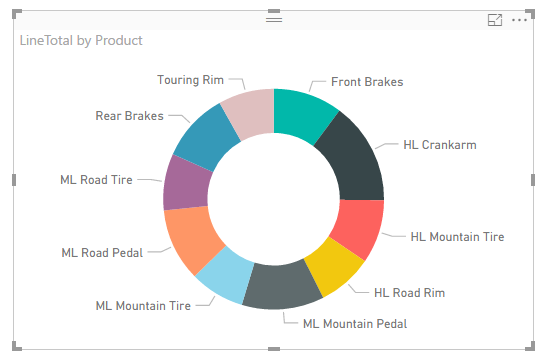
\includegraphics[width=14cm]{IMG/30.png} 
\end{center}

\begin{center}
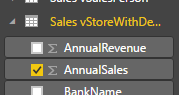
\includegraphics[width=7cm]{IMG/31.png} 
\end{center}
16. En el panel Campos, bajo Sales vStoreWithDemographics, hacer click y arrastrar el campo AnnualSales
directamente al area de reportes. Verificar como se crea automaticamente un grafico de barras.\\\\
\begin{center}
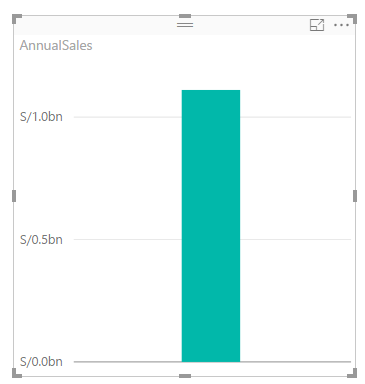
\includegraphics[width=9cm]{IMG/32.png} 
\end{center}
17. En el panel Campos, seleccionar la casilla de verificacion de AnnualRevenue, y apreciar que este adiciona el
campo al grafico de barras.\\\\
\begin{center}
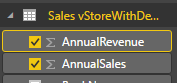
\includegraphics[width=11cm]{IMG/33.png} 
\end{center}
18. En el panel Campos, hacer click en la elipsis contigua a AnnualRevenue, y hacer click en Renombrar
(Rename). Tipear Beneficios anuales luego presionar Enter.\\\\
\begin{center}
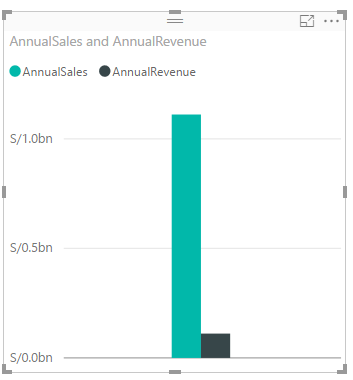
\includegraphics[width=11cm]{IMG/34.png} 
\end{center}

\begin{center}
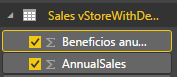
\includegraphics[width=11cm]{IMG/35.png} 
\end{center}
19. Repetir el paso 18, para renombrar el campo AnnualSales a Ventas Anuales. Apreciar que los nombres en
los titulus y leyenda del grafico de barras se han actualizado.\\\\
\begin{center}
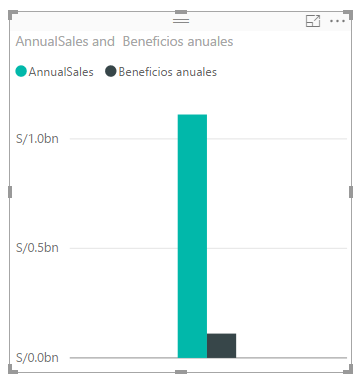
\includegraphics[width=11cm]{IMG/36.png} 
\end{center}
\begin{center}
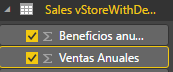
\includegraphics[width=11cm]{IMG/37.png} 
\end{center}
\begin{center}
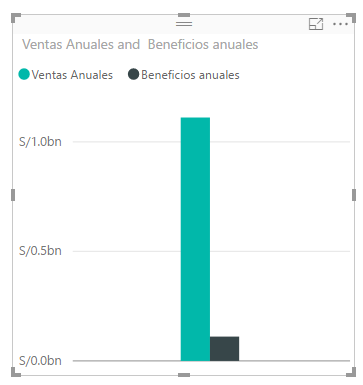
\includegraphics[width=11cm]{IMG/38.png} 
\end{center}
20. Hacer click en el area de reporte, luego en el panel de Visualizaciones y en la pestana Formato (Format).\\\\
\begin{center}
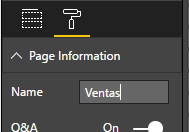
\includegraphics[width=9cm]{IMG/39.png} 
\end{center}
21. Expandir la Informacion de pagina (Page Information), y en la casilla Nombre tipear Ventas. Hacer click en el
area de reporte y apreciar que el nombre ha cambiado en la pestana al final del reporte.\\\\
\begin{center}
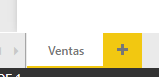
\includegraphics[width=9cm]{IMG/40.png} 
\end{center}
22. En el menu Archivo (File menu), hacer click en Guardar (Save), crear un directorio Power BI, y guardar el
archive como Ventas de Adventure Works Sales.\\\\
Parte 3: Publicar el reporte en el portal de Power BI\\\\
1. En el menu principal (Home ribbon), hacer click en Publica (Publish).\\\\
\begin{center}
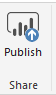
\includegraphics[width=4cm]{IMG/a.png} 
\end{center}
2. Si pregunta por Guardar los cambios, hacer click en Guardar (Save).\\\\
3. En la ventana de Power BI Desktop, ingresar la direccion de correo electronico de su cuenta Microsoft y
luego hacer click en Iniciar Sesion (Sign in).\\\\
4. En la Ventana de Iniciar Sesion (Sign in) con su cuenta, ingresar la contrasena y luego hacer click en Iniciar
Sesion (Sign in).\\\\
\begin{center}
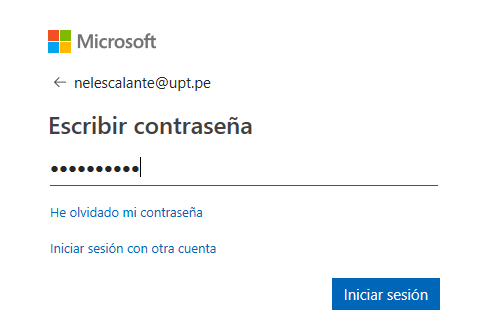
\includegraphics[width=11cm]{IMG/b.png} 
\end{center}
5. El reporte sera publicado en el Portal de Power BI. Cuando la ventana muestre Satisfactorio (9Success), hacer
click en Abrir (Open) 'Ventas Adventure Works.pibx' en Power BI para ver el reporte en linea.\\\\
\begin{center}
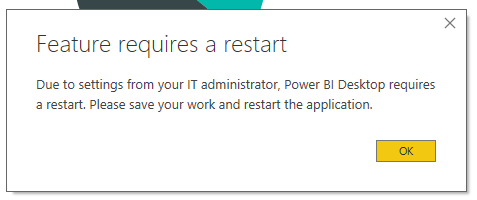
\includegraphics[width=12cm]{IMG/c.png} 
\end{center}
\begin{center}
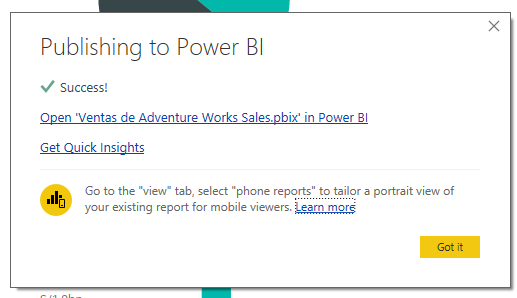
\includegraphics[width=12cm]{IMG/d.png} 
\end{center}
6. Cuando el navegador se abra, hacer click en Iniciar Sesion, ingresar su correo y contrasena, Iniciar sesion, y
esperar a que el reporte abra en Internet Explorer.\\\\
\begin{center}
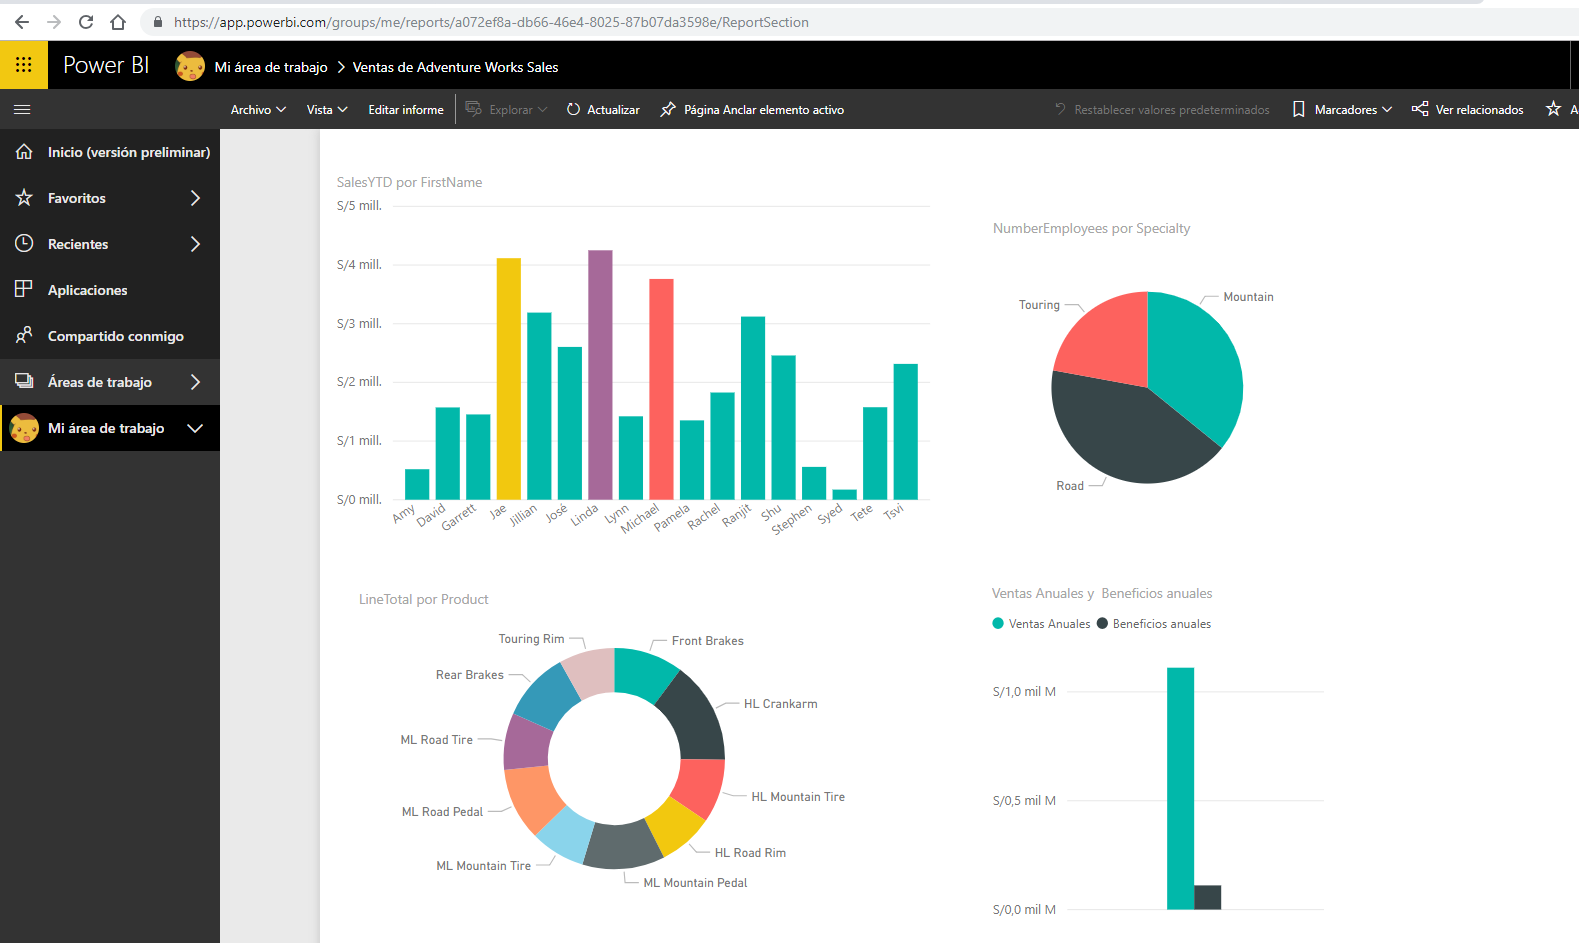
\includegraphics[width=18cm]{IMG/e.png} 
\end{center}



\end{document}